%!TEX root = ../thesis.tex
%*******************************************************************************
%****************************** Third Chapter **********************************
%*******************************************************************************
\chapter{Topology of the Lattice}\label{chapter:Topology}

% **************************** Define Graphics Path **************************
\ifpdf
    \graphicspath{{Chapter3/Figs/Raster/}{Chapter3/Figs/PDF/}{Chapter3/Figs/}}
\else
    \graphicspath{{Chapter3/Figs/Vector/}{Chapter3/Figs/}}
\fi
QCD presents two key properties that distinguish it from the other forces of nature:
\begin{enumerate}
\item Confinement of quarks, resulting in the absence of isolated quarks.
\item Dynamical chiral symmetry breaking, leading to dynamical generation of mass. This results in a substantial discrepancy between the mass of hadrons and the sum of the masses of the quarks that comprise them.
\end{enumerate}
These properties have been observed experimentally, however the question of how they arise from the gauge theory of QCD outlined in the preceding chapter is still the subject of intense investigation. It is believed that both these properties are connected by some underlying topological structure of the QCD vacuum. Proposed candidates include Abelian monopoles~\cite{tHooft:1981bkw,Smit:1989vg,Matsubara:1993nq,Suzuki:1989gp,Mandelstam:1974pi,Kronfeld:1987ri,Ivanenko:1990xu, Chernodub:1995tt}, instantons~\cite{Belavin:1975fg,Witten:1978bc,Callan:1977gz,Schafer:1996wv,Trewartha:2013qga,Aharonov:1978jd} and centre vortices~\cite{'tHooft:1977hy,'tHooft:1979uj,Feynman:1981ss,Aharonov:1978jd,Cornwall:1979hz,Nielsen:1979xu,Mack:1978rq}. With the advent of lattice simulations, the most promising of these appears to be the centre vortex model. Numerical evidence from the lattice has been amassed that indicates that topological objects known as centre vortices are tied to both confinement and dynamical chiral symmetry breaking~\cite{Biddle:2018dtc,Faber:1997rp,Langfeld:1998cz,Bowman:2008qd,Trewartha:2015ida,Trewartha:2015nna,Trewartha:2017ive,DelDebbio:1996lih,Greensite:2003bk,DelDebbio:1998luz,OMalley:2011aa,Langfeld:2003ev,Bowman:2010zr}. It is therefore the subject of this research to further extend the investigation into the properties of centre vortices, specifically in the gluonic sector of QCD.\\

As dynamical chiral symmetry breaking is primarily concerned with quarks, we will omit a detailed discussion of this property and instead begin this chapter outlining the confinement property exhibited by the strong force. We will then introduce centre vortices and motivate how they provide a potential explanation for confinement in QCD. From here we will describe how it is that we can identify centre vortices on the lattice, and survey the lattice results found in current literature pertaining to centre vortices. Finally we will briefly describe instantons and topological charge, in preparation for later chapters that draw on these concepts.  

\section{Confinement}\label{sec:Confinement}
The confinement property of QCD, and the accompanying notion of asymptotic freedom, is one of the defining low-energy features of the theory of the strong interaction. After Gell-mann and Zweig's concurrent proposal of quarks as the elementary constituents of baryons and mesons~\cite{GellMann:1964nj,Zweig:1964jf}, it was natural to then attempt to observe these new particles in isolation. However, efforts to observe quarks proved impossible. Early experiments testing the behaviour of electron-proton collisions demonstrated that protons scatter elastically, behaving as though they are finite-sized particles recoiling electromagnetically from the incident electron~\cite{Hofstadter:1956qs}. These experiments indicated no further substructure to the proton, inconsistent with the quark model. As accelerator energies improved, later experiments~\cite{Bloom:1969kc, Breidenbach:1969kd}, using electron energies of $7$ and $10~\si{GeV}$ found that inelastic scattering effects became dominant, with electrons behaving as though they were scattering off of loosely bound constituent particles. To explain this behaviour, Feynman proposed what is known as the 'parton' model~\cite{Feynman:1969ej}, treating the proton as being comprised of non-interacting electrically charged particles in the limit that the incident electron energy tends towards infinity. This is precisely the notion of asymptotic freedom; at large distance scales the partons are tightly bound, whereas at short distances they behave as free particles. It did not take long for the separate theories of quarks and partons to recognised as complementary, and by the early 70's the quark-parton model of hadrons accurately explained the the experimental results observed in particle colliders.\\

These experimental and theoretical results led in part to the development of the non-Abelian gauge field theory of QCD, as introduced in Chapter~\ref{chapter:LatticeQCD}. The proof that non-Abelian gauge theories are asymptotically free was discovered in 1973~\cite{Gross:1973id}, and experimental evidence of the existence of 3 quark colours through study of the cross section of $e^+ e^-$ collisions supports the initial $SU(3)$ colour symmetry anticipated by Gell-Mann and Zweig. At high energies, QCD has consistently explained the behaviour of hadronic matter, and has become the accepted theory of the strong nuclear interaction. However, the question of whether QCD is indeed a confining theory still remains. As confinement is a low-momentum property of QCD, it is apparent that any analytic proof of confinement must take place far from the asymptotic limit. To date, no such analytic proof has been found.\\

Lattice calculations are currently the only method by which it is possible to investigate low-energy QCD phenomena from first-principles. Calculations of the static potential between two massive quarks, both recent and old~\cite{Born:1993cq, Bonnet:1999gt, Creutz:1980hb, DiGiacomo:1990hc}, have shown that the potential rises linearly at sufficiently large separation distances. This behaviour is precisely what is expected of a colour confining theory. Other confinement mechanisms have also been proposed on the lattice, including mechanisms based on the behaviour of the gluon propagator at $q=0$~\cite{Zwanziger:1991gz} and the behaviour of the pion mass and Polyakov loop at light quark masses~\cite{Iwasaki:1991mr}. All lattice results so far have indicated that QCD is in fact a confining theory at low energy.\\

There is good evidence that confinement has its roots in the topological properties of the QCD vacuum. It is well understood that the QCD vacuum, unlike the QED vacuum, admits non-trivial instanton solutions: solutions of the vacuum field configurations that are all minima of the classical action, yet are distinguished from one another by a topological quantum number~\cite{Belavin:1975fg}. The presence of instanton solutions was significant in resolving the $U(1)$ anomaly~\cite{tHooft:1986ooh}, and provides an excellent method of calculating the ground state hadron spectrum~\cite{Schafer:1996wv}. The non-trivial topology of the QCD vacuum, and the success of topological features in resolving QCD anomalies, motivates the search for a topological explanation of confinement. 

\section{Centre Vortices}
Originally proposed by 't Hooft in 1978~\cite{'tHooft:1977hy,'tHooft:1979uj}, centre vortices are closed two-dimensional surfaces present in four-dimensional Euclidean space that carry colour-magnetic flux. The key property of a centre vortex is that in three dimensions, where the vortices appear as closed tubes, any Wilson loop (see Sec.~\ref{sec:LatticeDiscretisation}) that encloses a vortex will acquire a centre phase, such that
%
\begin{equation}
W(C)\rightarrow z \,W(C)\, ,
\end{equation}
%
where $z$ is a non-trivial element of $Z(3)$, the centre of $SU(3)$. The centre of a group is the subgroup that contains all the elements of the group that commute with all other elements. In the case of $SU(3)$ this corresponds to
%
\begin{equation}
Z(3) = \big\lbrace \exp\left(\frac{m 2\pi i}{3} \right)I ~ | ~ m = 0,\pm 1\big\rbrace\, . 
\end{equation}
%
Thus, the non-trivial elements of $Z_3$ are $z = \exp\left(\frac{\pm 2\pi i}{3}\right)I$. In the centre vortex model, it is therefore natural to refer to a vortex as being a `$+1$' or `$-1$' vortex, corresponding to the sign of the centre phase. When considering the value of any given Wilson loop, the centre vortex model suggests that
%
\begin{equation}
W(C) = \prod_i z_i\times W_0(C)\, ,
\end{equation}
%
where the $z_i$ correspond to the phases of the centre vortices intersecting the loop $C$, and $W_0(C)$ encapsulates the short-distance physics. A simple visualisation of this idea is shown in Fig.~\ref{fig:CentreVortex}. It is not immediately apparent why this form of the Wilson loop is related to confinement, however a simple $SU(3)$ calculation motivates the relevance of this model~\cite{Greensite:2016pfc}. To understand the significance of this calculation it is worth first deviating slightly to detail the relationship between the Wilson loop and the potential energy between two massive (static) quarks.\\
% 
\begin{figure}
\centering
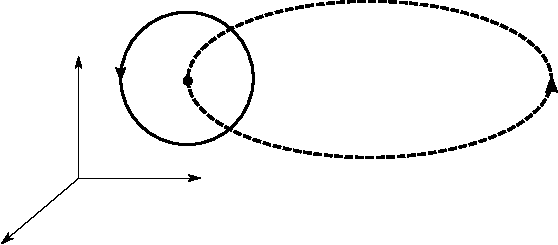
\includegraphics[width=\linewidth]{./centre_vortex.pdf}
\caption{\label{fig:CentreVortex} A single centre vortex (dashed line) intersecting a Wilson loop (solid line) in 3 dimensions. The Wilson loop will acquire a centre phase corresponding to the phase of the vortex.}
\end{figure}
%

Follwing the argument presented in Ref.~\cite{Makeenko:2009dw}, consider a Wilson loop calculated around a rectangle in the $x-t$ plane with dimensions $R\times T$. As the Wilson loop is gauge invariant, we are free to select a convenient gauge in which to perform the calculation. To this end, we choose the fields to be in axial gauge, such that $A_0(x)=0\implies U_0(x) = 1\,\forall\,x$. So the Wilson loop becomes
%
\begin{equation}
W(R\times T) = \Tr \left(U_1(0)\,U_1^\dagger(T)\right)\, .
\end{equation}
%
We can insert a complete set of energy eigenstates, $\sum_n |\,n\rangle\,\langle n \,|=1$ to obtain
%
\begin{align*}
W(R\times T) &= \Tr \left( \sum_n \langle U_1(0)\, |\, n\rangle\,\langle n\, |\, e^{-E_n(R)\, T}\, | \, U_1(0) \rangle\right)\\
&=  \sum_n \Tr \left( \big|\langle U_1(0)\, |\, n\rangle\big|^2 \right)\,e^{-E_n(R)\,T} \, .
\end{align*}
%
As $T\rightarrow \infty$, the only surviving contribution will be the lowest energy, $E_0(R)$. This means that
%
\begin{equation}
\lim_{T\rightarrow \infty} W(R\times T) \propto e^{-E_0(R)\, T}\, .
\label{eq:WilsonEnergy}
\end{equation}
The quantity $E_0(R)$ is the static quark potential, and if it is linear than its slope is referred to as the `string tension', $\sigma$.
\\

With Eq.~\ref{eq:WilsonEnergy} in mind, we return to the aforementioned $SU(3)$ confinement model. Consider a two-dimensional plane of area $L^2$, with $2N$ vortices piercing the plane. Assuming an even distribution of vortices, the total vortex density is $\rho = \frac{2N}{L^2}$. As there are two $SU(3)$ vortex types, corresponding to the two non-trivial phases, $z=\exp\left(\frac{\pm 2\pi i}{3}\right)$, we assume that there is an equal distribution of vortex phases, i.e. there are $N$ vortices of each type. The probability of finding $n$ vortices of a given phase in some region of the plane $A\subset L^2$ is equal to the probability that exactly $n$ vortices are in $A$, multiplied by the probability that exactly $N-n$ vortices are outside of $A$, multiplied by a combinatoric factor. Expressed mathematically, this is
%
\begin{equation}
P_N(n) = {N\choose n} \left(\frac{A}{L^2}\right)^n \left(1-\frac{A}{L^2}\right)^{N-n}\, .
\end{equation}
%
The expectation value of the Wilson loop around the perimeter of $A$ can be written as
%
\begin{equation}
\langle W(\partial A)\rangle = \sum_{m,n = 0}^N \left(\exp\left(\frac{2\pi i}{3}\right)\right)^n P_N(n)\, \left(\exp\left(-\frac{2\pi i}{3}\right)\right)^m P_N(m)\, .
\end{equation}
%
If we assume the vortex phases are uncorrelated, then we can make use of the following property of uncorrelated random variables $X$ and $Y$,
%
\begin{equation}
E[XY] = E[X]\, E[Y]\, ,
\end{equation}
%
to write
%
\begin{equation}
\langle W(\partial A)\rangle = \sum_{n=0}^N \left(\exp\left(\frac{2\pi i}{3}\right)\right)^n P_N(n)\,\sum_{m=0}^N \left(\exp\left(\frac{2\pi i}{3}\right)\right)^m P_N(m)\, .
\label{eq:WilsonExpectation}
\end{equation}
%
We consider just the first sum in Eq.~\ref{eq:WilsonExpectation} and calculate
%
\begin{align*}
\sum_{n=0}^N \left(\exp\left(\frac{2\pi i}{3}\right)\right)^n P_N(n) & = \left(1-\frac{A}{L^2}\right)^{N}\sum_{n=0}^{N} {N\choose n} \left(\exp\left(\frac{2\pi i}{3}\right)\,\frac{A}{L^2}\left(1-\frac{A}{L^2}\right)^{-1}\right)^n\\
&=\left(1+\left(\exp\left(\frac{2\pi i}{3}\right) - 1\right)\frac{A}{L^2}\right)^N\, ,
\end{align*}
%
where we have made use of the binomial series to evaluate the sum. Hence the total expectation value is
%
\begin{align}
\langle W(\partial A)\rangle &=\left(1+\left(\exp\left(\frac{2\pi i}{3}\right) - 1\right)\frac{A}{L^2}\right)^N\, \left(1+\left(\exp\left(\frac{-2\pi i}{3}\right) - 1\right)\frac{A}{L^2}\right)^N\nonumber\\
&=\left(1 -3\frac{A}{L^2} + 3\left(\frac{A}{L^2}\right)^2\right)^N\nonumber\\
&= \left(\left(\frac{A}{L^2}\right)^3+\left(1-\frac{A}{L^2}\right)^3\right)^N\, .\label{eq:WilsonExpectationSimple}
\end{align}
%
Rewriting Eq.~\ref{eq:WilsonExpectationSimple} in terms of the vortex density $\rho$, we have
%
\begin{equation}
\langle W(\partial A)\rangle = \left(\left(\frac{A\rho}{2N}\right)^3+\left(1-\frac{A\rho}{2N}\right)^3\right)^N\, .
\end{equation}
%
Now we take the limit as $N,L^2\rightarrow\infty$, keeping $\rho$ constant. Taking the limit, we find
%
\begin{equation}
\langle W(\partial A)\rangle = \exp\left(-\frac{3}{2}\rho A\right)
\label{eq:WilsonAreaLaw}
\end{equation}
%
Letting $A=R\times T$ as in Eq.~\ref{eq:WilsonEnergy}, we see that $E_0(R) = \frac{3}{2}\rho R$, so the static quark potential rises linearly with string tension $\sigma = \frac{3}{2}\rho$, exactly as it should in a confining theory. Eq.~\ref{eq:WilsonAreaLaw} demonstrates an {\it area law} behaviour of the Wilson loop; this is often taken as a requirement for confinement~\cite{DelDebbio:1998luz,Dosch:1988ha}. We see then that we have, from a set of simple assumptions, constructed a model that exhibits confinement.\\

It is important to highlight the assumptions and simplifications made in the above argument. Most easily addressed is the assumption that there is an equal number of $+1$ and $-1$ vortices. By identifying vortices in Monte-Carlo generated configurations and plotting the distribution of phases in Fig.~\ref{fig:VortexDistribution}, we see that there is little deviation from an even distribution, especially in the ensemble average. This is an expected result, as vortices are tubes of chromo-magnetic flux, and thus must satisfy the Bianchi identity. In the absence of spontaneous symmetry breaking, this requirement is analogous to the electrodynamics condition $\nabla \cdot B = 0$, so we see that the flux line cannot terminate, and thus the tubes must be closed. Hence, over all space, we would expect that every $+1$ vortex is accompanied by a $-1$ vortex arising from the tube piercing the same plane in the opposite direction. On the lattice we observe a slight deviation from this idealised condition due to vortices being closed by lattice periodicity, but it is apparent that on average there is no preferred phase.\\
%
\begin{figure}[h]
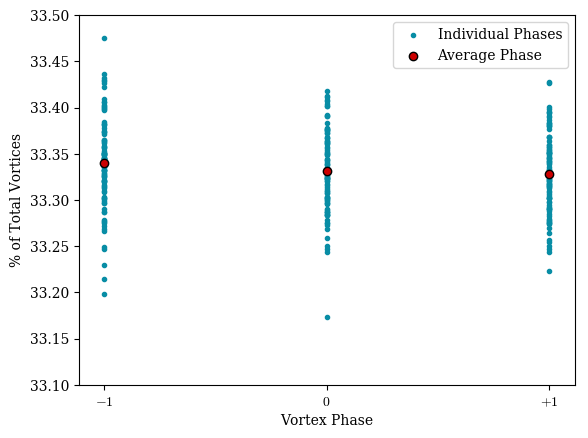
\includegraphics{./VortexDistribution.png}
\caption{\label{fig:VortexDistribution}A plot of the vortex phase distribution of 100 Monte-Carlo generated configurations, as a percentage of the total number of vortices. The method by which vortices are identified will be detailed in Sec.~\ref{sec:LocatingVortices}.}
\end{figure}
%

The assumption that the vortex density is constant is, however, less well motivated. So far we have treated vortices as infinitesimally thin sheets in 4D, which is not physically motivated. An infinitely thin vortex introduces a singularity in the action, as the vortex flux must be constrained to an infinitely thin cross-section. Rather, physical vortices are `thick'; they have a finite cross-section in the direction perpendicular to the vortex sheet. If the vortex is contained entirely within the area $A$ it contributes the centre phase as described above. However, as $A$ approaches the size of the vortex cross section, one must account for vortices that are only partially inside $A$, and thus not necessarily contributing a pure centre phase. Although this consideration spoils the elegance of the above confinement mechanism for small Wilson loops, it does potentially save the model from a previously noted pitfall related to the Casimir scaling of the Wilson loop expectation value~\cite{Greensite:1982be,Faber:1997rp}, as will be described in more detail in Sec.~\ref{sec:CurrentEvidence}. Finally, it is worth noting that this issue is only relevant to Wilson loops of similar size to the vortex cross-section. As the Wilson loop increases in size, the majority of the vortices will be contained entirely within the loop, with a diminishing number of thick vortices overlapping the perimeter of the loop, as shown in Fig.~\ref{fig:VortexSizes}.\\
%
\begin{figure}[htb!]
\centering
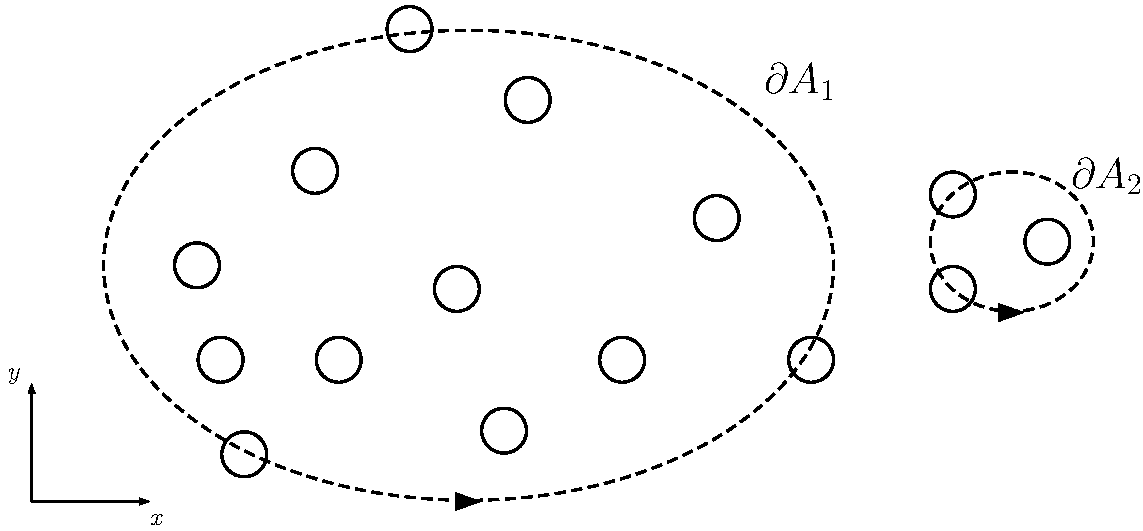
\includegraphics[width=\linewidth]{./LargeVortex.pdf}
\caption{\label{fig:VortexSizes}An example of two Wilson loops (dashed lines) lying in a plane, pierced by vortices of finite cross-section (solid lines). \textbf{Left:} The majority of vortices contributing to the phase are fully contained within the large loop, with only a few overlapping at the perimeter. \textbf{Right:} For a small loop, the contribution from overlapping vortices is significant as there are few vortices fully inside the loop.}
\end{figure}

The final assumption is that the vortex locations are random and uncorrelated from one another. This is perhaps the most significant assumption made in the above picture, as can be seen from the following calculation~\cite{Engelhardt:1999fd}. As vortices must form closed lines in 3D, let us suppose that instead of being randomly distributed, the vortices come in pairs separated by a maximum distance $d$. This corresponds to requiring that vortex lines form a closed loop of some maximum diameter $d$. If this vortex line pierces the Wilson loop in both directions, then the product of the phases, $\exp\left(\frac{2\pi i}{3}\right)\times \exp\left(\frac{-2\pi i}{3}\right) = 1$, results in no contribution to the Wilson loop. Hence, the only vortices capable of contributing a non-trivial phase to the Wilson loop are those contained within a strip of width $d$ about the perimeter of the loop. Note that not every vortex within this strip will contribute a non-trivial phase, as the vortex may be smaller than $d$ or oriented such that the vortex flows in direction of $\partial A$ and thus still pierces twice. We will take the most generous case, however, and assume that every vortex piercing this strip contributes a non-trivial phase. To first order, the area of relevance to to the expectation value of the Wilson loop is now $A_\text{strip}=\partial A\, d$. The probability to find $N$ vortices lying within this strip is 
%
\begin{equation}
P_N(n) = {N\choose n} \left(\frac{\partial A d}{L^2}\right)^n \left(1-\frac{\partial A d}{L^2}\right)^{N-n}\, .
\end{equation}
%
By following the same steps used to arrive at Eq.~\ref{eq:WilsonAreaLaw}, we find
%
\begin{equation}
\langle W(\partial A)\rangle = e^{-\frac{3}{2}\rho\, d\, \partial A}\, .
\end{equation}
%
So we see that instead of an area law, we now have a perimeter law for the Wilson loop, dependent on the upper bound for the vortex size. This implies that if there is some upper limit on the size of a vortex, we can no longer expect to see confining behaviour. We therefore deduce that to obtain a confining theory, it is necessary to allow the vortex size to be potentially infinite. In the language of the vortex model, this is called \textit{vortex percolation}. Conversely, the presence of an upper bound on the vortex size would imply a deconfined phase. This suggests that the size of vortices can be used as an \textit{order parameter} for confinement~\cite{Langfeld:1998cz}, with two distinct phases:
\begin{enumerate}
\item Vortex percolation $\implies$ confinement.
\item Loss of vortex percolation $\implies$ deconfinement.
\end{enumerate}

\subsection{Locating Centre Vortices}\label{sec:LocatingVortices}
Now that we have motivated the case for the centre vortex model, we wish to consider how it is that we identify vortices on a lattice configuration. The guiding principle behind the method we employ is that we wish to find some way to distinguish between a configuration containing vortices, and the same configuration with the vortices removed. Note that the vortex-free configuration is not necessarily trivial; it will still contain all the short distance physics we wish to ignore. We should therefore discuss how it is that a vortex can be inserted into a configuration to first build up a picture of what it is that separates a configuration containing vortices from one that does not.\\

We know from the previous section that our vortex insertion must result in a transformation of the Wilson loop containing the vortex such that
%
\begin{equation}
W(C)\rightarrow z W(C),~z = \exp\left(\frac{\pm2\pi i}{3}\right)\, .
\end{equation} 
%
It should be apparent that this behaviour is not possible from an ordinary gauge transformation, as the Wilson loop is a gauge invariant quantity. There is an infinite class of gauge transformations that can result in this behaviour, but the key property connecting them is that they are \textit{singular}~\cite{'tHooft:1977hy}. This means that the transformations associate the same point in space with two different values. For example, consider a gauge potential $A_\mu$ undergoing a gauge transformation $\Omega$ around a closed circle $C$. Let $\theta$ be the angular coordinate, and define the gauge transformation
%
\begin{equation}
\Omega(\theta) = \exp\left(-i\theta Q\right),~\theta\in [0,2\pi]\, ,
\label{eq:SingularGT}
\end{equation}
%
where
%
\begin{equation}
Q = \frac{1}{2}\lambda_3 +\frac{1}{2\sqrt{3}}\lambda_8 = \frac{1}{3}\diag\left(2,-1,-1\right)\label{eq:Q}
\end{equation}
As $\Omega(0) \neq \Omega(2\pi)$, the transformation is singular. According to Eq.~\ref{eq:LinkTransformation} the gauge link around the path, $U(x(\theta),\theta=0)$, then becomes
%
\begin{equation}
U(x(\theta),\theta=0) \rightarrow \Omega(2\pi)\,U(x(\theta),\theta=0)\,\Omega(0)\, ,
\end{equation}
%
with the corresponding Wilson loop
%
\begin{align}
W_0(C(\theta)) &\rightarrow \Tr\left( \Omega(2\pi)\,U(x(\theta),\theta=0)\,\Omega(0)\right)\\
&=\Tr\left(\exp\left(\frac{2\pi i}{3}\right)U(x(\theta),\theta=0)\right)\\
&=\exp\left(\frac{2\pi i}{3}\right)\,W_0(C(\theta))\, .
\end{align}
We see that through the use of a singular centre transformation we have introduced a  centre vortex to the configuration. Note that the transformation in Eq.~\ref{eq:SingularGT} is not unique, and if written in Cartesian coordinates the singular nature is replaced by a pole at the centre of the circle. The literature makes use of both these definitions of the vortex gauge transformation~\cite{'tHooft:1977hy,Faber:1999gu}. As our vortex depends only on the angular coordinate, this vortex is infinitely thin, as any size Wilson loop will acquire the vortex flux. Transformations creating thick vortices by adding a radial profile to the singular gauge transformation have been explored in Ref.~\cite{Faber:1997rp}. On the lattice, this gauge transformation corresponds to multiplying a single link $U_\mu(x)$ by the centre phase $\exp\left(\frac{2\pi i}{3}\right)$, such that the plaquettes associated with this link are multiplied by the same centre phase, creating in 3D a $1\times 1$ vortex, as seen in Fig.~\ref{fig:CreatedVortex}. Larger vortices are created by multiplying more links by the same centre phase. This suggests that we can consider our gauge links to be of the form
%
\begin{equation}
U_\mu(x) = Z_\mu(x)\,R_\mu(x)\, ,
\label{eq:VortexDecomposition}
\end{equation}
%
where $Z_\mu(x)$ is the `vortex-only' field consisting of centre elements, and $R_\mu(x)$ is the background `vortex-removed' field.\\
%
\begin{figure}[htb!]
\centering
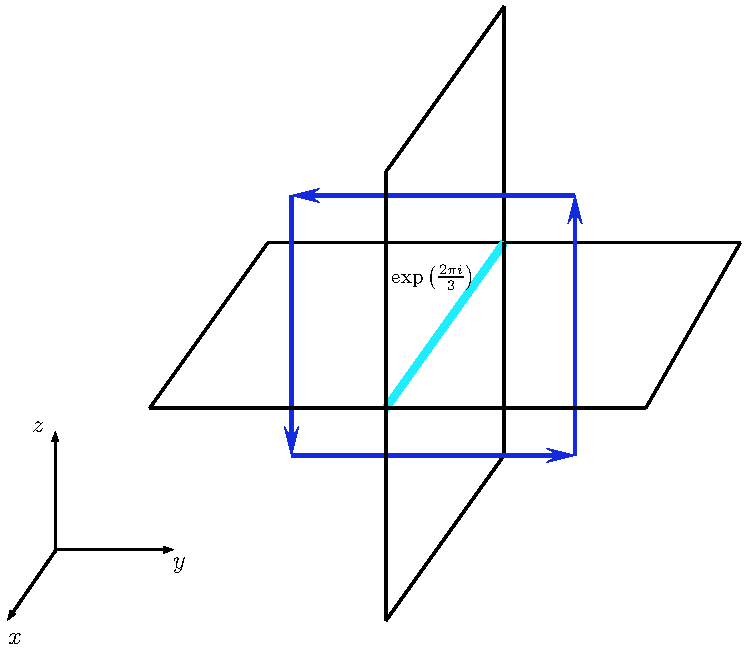
\includegraphics[width=0.7\linewidth]{./CreatedVortex.pdf}
\caption{\label{fig:CreatedVortex} A $1\times 1$ vortex (blue) created by multiplying the centre link (cyan) by a centre phase. Note that there are two more plaquttes in the time direction that have been suppressed, which serve to make the vortex a cube in 4D.}
\end{figure}
%

With the understanding that a configuration containing vortices differs from one that doesn't by a singular gauge transformation, we should consider the \textit{adjoint representation} of $SU(3)$, as it has the property of being invariant under centre transformations. The adjoint representation is defined such that any $SU(3)$ element in this representation can be written in the form $U^A_\mu(x) = \exp\left(i \omega_k(x) f^k\right)$, where $f^k$ are the $8\times 8$ $SU(3)$ structure constants. These constants are given by the Lie algebra relationship
%
\begin{equation}
\left[\frac{\lambda_i}{2},\,\frac{\lambda_j}{2}\right] = i\sum_k f_{ij}^{k}\frac{\lambda_k}{2}\, .
\end{equation}
%
To transform the gauge links $U_\mu(x)$ from the fundamental representation to the adjoint representation, it is necessary to find a mapping $D:SU(3)^\text{F}\rightarrow SU(3)^A$ that preserves the group operation. This means that for any $U,\,V \in SU(3)^F$, then we require that
%
\begin{equation}
D(U\,V) = D(U)\,D(V)\, .
\label{eq:RepMap}
\end{equation}
%
Consider the mapping
%
\begin{equation}
\left[U_\mu^A(x)\right]_{ij} = \left[D(U_\mu(x))\right]_{ij} = \frac{1}{2}\Tr\left(\lambda_i \, U_\mu(x) \, \lambda_j\, U_\mu(x)^\dagger\right)\, .
\label{eq:AdjointRep}
\end{equation}
%
This mapping satisfies Eq.~\ref{eq:RepMap} (see Appendix \ref{app:RepMapProof}), and it is easy to see that if $U_\mu(x)\rightarrow Z_\mu(x)\, U_\mu(x)$ for $Z_\mu\in Z_3$ then $U^A_\mu(x)$ is unchanged. This means that the adjoint representation is invariant under singular centre transformations (or, more generally, any centre transformation) and is therefore insensitive to the presence of vortices in a given configuration. Considering the decomposition of $U_\mu(x)$ into vortex-only and vortex-removed components presented in Eq.~\ref{eq:VortexDecomposition}, we see that in the adjoint representation, 
%
\begin{equation}
U_\mu^A = R_\mu^A\, .
\end{equation}
%
It is then clear that the adjoint representation can be utilised to isolate the background vortex-removed field. This property is key to the vortex identification procedure described below.
 
\subsubsection{Maximal Centre Gauge}\label{sec:MCG}
We now turn to the choice of gauge used to identify vortices in the fundamental representation. Known as maximal centre gauge, this gauge serves to bring each gauge link on the lattice as close as possible to a centre element, such that
%
\begin{equation}
\left\| U _ { \mu } ^ { \Omega } ( x ) - Z _ { \mu } ( x ) \right\|\, ,
\end{equation}
%
is minimised. There are numerous implementations of this gauge~\cite{Montero:1999by,Faber:1999sq}, however we choose to implement it by maximising the ``mesonic'' functional~\cite{Langfeld:2003ev}
%
\begin{equation}
R = \frac { 1 } { V N _ { \operatorname { dim } } n _ { c } ^ { 2 } } \sum _ { x , \mu } \left| \operatorname { Tr } U _ { \mu } ^ { G } ( x ) \right| ^ { 2 }\, ,
\label{eq:MCGFunctional}
\end{equation} 
%
where $VN _ { \operatorname { dim } }$ is the number of links on the lattice, and $n_c=3$ is the number of colours. At first glance it is unclear why this gauge would assist in isolating vortices. To elucidate the connection, we consider the trace of the adjoint gauge link $U^A_\mu(x)$ obtained from Eq.~\ref{eq:AdjointRep},
%
\begin{equation}
\Tr\left(U^A_\mu(x)\right) = \left|\Tr\left(U_\mu(x)\right)\right|^2 - 1\, .
\end{equation}
%
The details of the above expression are given in Appendix \ref{app:RepMapProof}. We see therefore that maximising Eq.~\ref{eq:MCGFunctional} is equivalent to maximising
%
\begin{equation}
R^A = \frac { 1 } { V N _ { \operatorname { dim } } n _ { c } ^ { 2 } } \sum _ { x , \mu } \left( \operatorname { Tr } U _ { \mu } ^ { A,\,G } ( x ) \right)\, .
\end{equation}
%
$R^A$ is clearly maximised when $U_\mu^A(x)=I$, which requires that $U_\mu(x) \in Z_3$. Thus, maximising $R^A$ is equivalent to bringing the vortex-removed field $R_\mu(x)$ as close as possible to the identity, which in the idealised case would take $U_\mu(x)\rightarrow Z_\mu(x)$. Of course, it is in general not possible to fully gauge-away the $R_\mu(x)$ field, but we assume that once $R$ is maximised the trace is sufficiently close to the centre phase $Z_\mu(x)$ that it identifies the centre element associated with this link. To then construct the vortex-only field, we simply project onto this nearest centre element. This projection step is not a gauge rotation, and naturally removes all the short-range physics, as we have essentially enforced a trivial background configuration. This projection gives us our three sets of configurations:
\begin{enumerate}
\item Original `untouched' fields, $U_{\mu}(x),$

\item Projected vortex-only fields, $Z_{\mu}(x),$

\item Vortex-removed fields, $R_\mu(x) = Z^{\dagger}_{\mu}(x)\,U_{\mu}(x).$
\end{enumerate}
These three sets will be collectively referred to as our vortex-modified configurations for the remainder of this research.\\

There are two primary assumptions related to this vortex identification method~\cite{Faber:1999gu}. The first is due to the degeneracy in the maxima of $R$, the so-called Gribov copy issue. This degeneracy results in it being unclear whether a given maxima is the global maxima, or merely local. If it is local, and far from the global maxima, then it is entirely possible that vortices will be misidentified. This is because the background vortex-removed field contribution could be far from the identity, resulting in an incorrect centre phase being obtained when the configuration is projected onto $Z_3$.\\

The second assumption is that the partitioning of $U_\mu(x)$ into $Z_\mu(x)$ and $R_\mu(x)$ is valid. In other words, we assume that the physical thick vortices are sufficiently small such that they can be defined by a series of single-link centre transformations on the lattice, like that shown in Fig.~\ref{fig:CreatedVortex}, rather than by a larger multiple-link transformation, as shown in Fig.~\ref{fig:MultipleLink}. This is equivalent to the discontinuity related to the vortex being larger than a single plaquette. If the vortices are too large, the MCG procedure becomes unable to contract their thickness such that they are identified by a single link.\\

Although these assumptions are potentially strict, numerical evidence has shown that if a vortex is inserted into a configuration by hand, then the above MCG procedure is capable of consistently identifying its location~\cite{Faber:1999gu,Montero:1999by}. This suggests that the required assumptions are valid to a fair degree, and thus we are motivated to continue to employ this vortex identification method. Furthermore, efforts to improve the obtained value of $R$ through use of simulated annealing~\cite{Bogolubsky:2009dc} or preconditioning~\cite{Cais:2008za} have found that the amount of identified vortices actually decreases as $R$ is increased, and the resulting phenomenology is worse overall. The proposed reasoning for this is that these improvement techniques have the property of increasing the size of vortices, resulting in an amplification of the issue raised above, in which the MCG procedure fails to identify large vortices. Hence, based on these prior findings, we do not attempt to escape the first Gribov region the MCG procedure finds itself in, as in the study of centre vortices it is appropriate to remain near this local maxima.
%
\begin{figure}[htb!]
\centering
\begin{tikzpicture}[scale=0.9]
\begin{scope}[very thick,decoration={
    markings,
    mark=at position 0.5 with {\arrow[scale=2]{stealth}}}
    ] 
  \draw[line width=1.0,postaction={decorate}](-4,-1.5)--node[above]{}(1.5,-1.5)node(f){};
  
  % z direction  
  \draw[line width=1.0]( 1.5,-1.5)--node[right]{} (1.5,4.0);    % width  3.25-(-1.5) = 4.75
  \draw[line width=1.0,postaction={decorate},color=cyan]( 1.5, 4.0)--node[above,color=black]{$\exp{\left(\pi i Q\right)}$}(-4.0,4.0);    % height 6.25-1.5    = 4.75
  \draw[line width=1.0,postaction={decorate}](-4.0, 4.0)--node[left]{}(-4.0,-1.5);
  
  \draw[line width=1.0,postaction={decorate}](1.5,-1.5) --(7,-1.5);
  \draw[line width=1.0,postaction={decorate}](7,-1.5) -- (7,4);
  \draw[line width=1.0,postaction={decorate},color=cyan](7,4) --node[above,color=black]{$\exp{\left(\pi i Q\right)}$} (1.5,4);

  \end{scope}
\end{tikzpicture}
\caption{\label{fig:MultipleLink} An example of a $2\times 1$ vortex, arising from a centre transformation split across two links (cyan). Each $1\times 1$ plaquette individually will not acquire a centre phase, but the the $2\times 1$ loop will.}
\end{figure}

\subsection{Current Evidence for Centre Vortices}\label{sec:CurrentEvidence}
Now that we have developed an understanding of centre vortices and how they are located, we can summarise briefly the current lattice evidence surrounding vortices and their relationship to various calculable quantities.
 
\subsubsection{String Tension}
As discussed previously, the string tension is the slope of the linear potential observed between two massive, static quarks. In $SU(2)$ studies, it has been shown that vortex removal results in a complete loss of the string tension, and on vortex only configurations it is possible to fully replicate it~\cite{Cais:2008za}. In $SU(3)$ the picture is less clear. Without smoothing (see Chapter~\ref{chapter:Smoothing}), it is only possible to regain $\sim 62\%$ of the original string tension on the vortex only configurations~\cite{Langfeld:2003ev}; however, under vortex removal the string tension vanishes just as in the $SU(2)$ case. Under smoothing, it is possible to achieve $\sim 97\%$ agreement, however the overall string tension on both the untouched and vortex only configurations is reduced to approximately $37\%$ of the original un-smoothed string tension~\cite{Trewartha:2015ida}.  

\subsubsection{Hadron Spectrum}
The low-lying hadron spectrum provides an excellent probe of the presence of dynamical chiral symmetry breaking. By comparing the masses of hadrons that would have degenerate mass if chiral symmetry is restored, we can observe whether dynamical mass generation effects are present. Through use of the overlap fermion action, it has been possible to show in $SU(3)$ that the vortex-only spectrum under a small amount of cooling closely follows the trends of the untouched hadron spectrum~\cite{Trewartha:2017ive}. The slight discrepancy can be attributed to the necessity of cooling when considering the vortex only configurations. On the vortex removed configurations, dynamical mass generation vanishes and hadrons with the same quark content once again become degenerate~\cite{Trewartha:2017ive}. This is a clear signal of the restoration of chiral symmetry. 

\subsubsection{Mass Function}
The mass function, $M(p)$, represents the observed mass of a quark as a function of momentum. Dynamical mass generation presents itself as an amplification of the low-momentum mass function, indicating an observed long-range mass that is greater than the bare mass of the quark. After 10 sweeps of cooling this amplification is indeed observed on both the vortex only and untouched mass function of $SU(3)$ configurations, whereas on the vortex removed mass function this amplification is greatly suppressed~\cite{Trewartha:2015nna}. In $SU(2)$, similar behaviour has also been observed~\cite{Bowman:2008qd}.

\subsubsection{Casimir Scaling}
Casimir scaling refers to the behaviour of the $SU(N)$ string tension in different representations (see e.g. the adjoint representation introduced in Sec.~\ref{sec:LocatingVortices}). As $N$ becomes increasingly large, it is found that the fundamental string tension $\sigma_F$ is related to the adjoint string tension $\sigma_A$ by $\sigma_A = 2\sigma_F$~\cite{Greensite:1982be}. Given our prior discussion of the adjoint representation, this should at first glance appear a surprising result, as we stressed that the adjoint representation is insensitive to the presence of vortices and thus the centre vortex model would suggest a vanishing string tension in the adjoint representation. However, numerical evidence shows that this is certainly not the case, even for $SU(2)$ and $SU(3)$~\cite{Ambjorn:1984mb,Ambjorn:1984dp,Campbell:1985kp}. This apparent contradiction can be resolved by considering vortices of finite thickness, as done in Ref.~\cite{Faber:1997rp}. This finite thickness manifests as a Wilson loop acquiring a vortex contribution of the form
%
\begin{equation}
G(x) = \Omega\,\exp\left(i \alpha_C(x)\,Q\right)\, \Omega^\dagger\,
\end{equation}
%
where $\Omega\in SU(3)$, $Q$ is as defined in Eq.~\ref{eq:Q} and $\alpha_C\in [0,2\pi]$ is a function satisfying
%
\begin{equation}
\alpha_C(x)=
\begin{cases}
0\, , &\, \text{Vortex lies entirely outside the Wilson loop of perimeter $C$}\\
2\pi\, , &\, \text{Vortex lies entirely inside the Wilson loop of perimeter $C$}\\
\end{cases}\, .
\end{equation}
%
Clearly for $\alpha_C(x) = 0,\,2\pi$ we recover the thin vortex behaviour, however the structure of $\alpha_C(x)$ away from these cases encodes a generalised vortex thickness. This thickness appears to resolve the Casimir scaling contradiction, and give the appropriate scaling behaviour for other representations of $SU(N)$ as well~\cite{Faber:1997rp}.
\subsubsection{Gluon Propagator}
The gluon propagator, $D(p^2)$, (see Chapter~\ref{chapter:GluonPropagator}) serves as an indicator of confinement. Similar to the mass function, low-momentum enhancement indicates non-perturbative behaviour. In both $SU(2)$ and $SU(3)$ it has been shown that vortex removal indicates a loss of this enhancement, suggesting a loss of confinement~\cite{Bowman:2010zr,Langfeld:2001cz,Quandt:2010yq}. However, vortex only results have not been previously calculated; these results are one of the main accomplishments of this research, and are presented in Chapter~\ref{chapter:GluonPropagatorResults}.

\section{Further Topological Quantities}
Although not the primary focus of this work, it is informative to  provide a definition for topological charge and introduce the notion of an instanton. Both these quantities provide a useful measure of the topological structure of the lattice, especially when we come to consider smoothing routines in Chapter~\ref{chapter:Smoothing}. Topological charge provides a simple numerical measure of the contribution of all topological objects. Furthermore, there is a connection between the location of topological charge and the geometry of centre vortices, specifically the intersection, touching and writhing points of centre vortices~\cite{Spengler:2018dxt,Reinhardt:2001kf}. Instantons are often used as the reference topological object in the literature~\cite{Moran:2008ra,Trewartha:2015ida}, with preservation of the instanton content of the lattice equated to a preserved topological structure.

\subsection{Topological Charge}\label{sec:TopQ}
The total topological charge is the `degree' of a particular field configuration, counting how many times $A_\mu$ covers the Lie algebra $\mathfrak{su}(3)$. Numerically, it is given by~\cite{Alexandrou:2017hqw}
%
\begin{equation}
Q = \int d^4x \frac { 1 } { 16 \pi ^ { 2 } } \epsilon _ { \mu \nu \rho \sigma } \operatorname { Tr } \left( F _ { \mu \nu } F _ { \rho \sigma } \right)\, \in\, \mathbb{Z} \, .
\label{eq:TopologicalCharge}
\end{equation} 
The term in the integrand is known as the topological charge density, denoted $q(x)$. From Eq.~\ref{eq:PlaquetteExpansion} it is clear we could evaluate $F_{\mu\nu}$ by taking the imaginary part of $P_{\mu\nu}$. However, it is common to make use of the clover leaf definition,
%
\begin{equation}
q_\text{clov}(x) = \frac{1}{16\pi^2} \epsilon _ { \mu \nu \rho \sigma } \Tr\left(C_{\mu\nu} \, C_{\rho\sigma}\right),
\end{equation}
%
where
\begin{equation}
C_{\mu\nu} = \frac{1}{4} \operatorname{Im}\left(P_{\mu\nu}(x) \, P_{\mu\nu}(x-\hat{\mu}) \, P_{\mu\nu}(x - \hat{\nu}) \, P_{\mu\nu}(x - \hat{\mu} - \hat{\nu})\right)\, .
\end{equation}
%
The clover-leaf loop combination is shown in Fig.~\ref{fig:Clover}. Much like the L\"uscher and Weisz action, we can expand this clover definition with larger combinations of loops to remove higher order errors. In our calculation of topological charge in Sec.~\ref{sec:TopChargeVis}, we employ a 5-loop improved topological charge, taking into account a linear combination of $1\times 1$, $2\times 1$, $2\times 2$, $2\times 3$ and $3\times 3$ clover loops~\cite{BilsonThompson:2001ca}.

\begin{figure}[htb!]
\centering
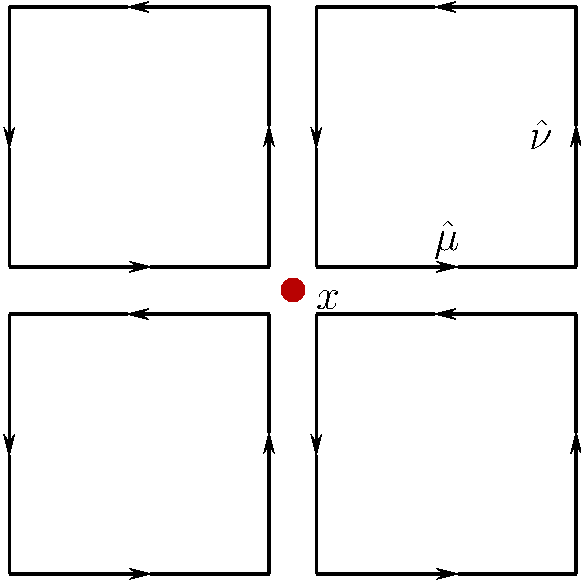
\includegraphics[width=0.5\linewidth]{./Clover.pdf}
\caption{\label{fig:Clover}The four plaquettes that compose the clover combination $C_{\mu\nu}$.}
\end{figure}

\subsection{Instantons}
The QCD vacuum is a non-trivial state, existing as a superposition of an infinite number of degenerate solutions enumerated by a topological quantum number. These solutions can be expressed as a gauge rotation from the trivial $A_\mu=0$ solution, such that
%
\begin{equation}
A_\mu = i(\partial_\mu \Omega)\,\Omega^\dagger\, .
\end{equation}
%
These are the so-called `pure gauge' configurations. For these vacuum configurations, the topological charge defined in Eq.~\ref{eq:TopologicalCharge} has a slightly modified interpretation; it now counts how many times the gauge transformation $\Omega(x)$ covers the group $SU(3)$. If we require that as $|x|\rightarrow \infty$, $A_\mu\rightarrow 0$, then  Eq.~\ref{eq:TopologicalCharge} becomes an integral of a total divergence and reduces to the Pontryagin number, calculated as an integral over the boundary of Euclidean space $S^3$~\cite{ryder1996quantum}
%
\begin{equation}
Q = \frac{1}{24\pi^2}\oint_{S^3} \epsilon_{\mu\nu\rho\sigma} \, \hat{\mu}\Tr\left(\left(\Omega^\dagger \,\partial_\nu \Omega\right)\,\left(\Omega^\dagger \,\partial_\rho \Omega\right)\,\left(\Omega^\dagger \,\partial_\sigma \Omega\right)\right)
\end{equation}
%
We wish to consider the potential tunnelling between different vacuum states, with a difference in topological charge $\Delta Q=1$. If we impose the condition
%
\begin{equation}
\int d^3x \,\left(q(t=\infty)-q(t=-\infty)\right)=1\, ,
\end{equation}
%
we can construct the gauge potential for a configuration inhabiting one vacuum at $t=\infty$, and another vacuum at $t=-\infty$. This solution for $A_\mu$ given these conditions is known as an instanton solution~\cite{Schafer:1996wv}. Unfortunately, there is no known analytic solution for an instanton in $SU(3)$. However, there is a known $\Delta Q=1$ instanton in $SU(2)$, known as the Belavin-Polyakov-Schwartz-Tyupkin (BPST) instanton solution~\cite{Belavin:1975fg}. It has the form
%
\begin{equation}
A_\mu(x) = \frac{2\eta_{a\mu\nu}\,x_\nu}{x^2+\rho^2}\,\frac{\sigma^a}{2}\, ,
\label{eq:InstantonSolution}
\end{equation}
%
where
%
\begin{equation}
\eta_{a\mu\nu} =
\begin{cases}
\epsilon_{a\mu\nu}\, , & \mu,\,\nu = 1,2,3\\
\delta_{a\mu}\, , & \nu=4\\
-\delta_{a\nu}\, , & \mu=4
\end{cases}\, ,
\label{eq:EtaSymbol}
\end{equation}
%
$\sigma^a$ are the Pauli matrices and $\rho$ is an arbitrary parameter known as the instanton radius. An anti-instanton solution corresponding to $\Delta Q=-1$ can be obtained by substituting $\eta$ with $\bar{\eta}$, where $\bar{\eta}$ is the same as Eq.~\ref{eq:EtaSymbol} but with a factor of $-1$ in the last two cases. The action associated with this configuration is 
%
\begin{equation}
S_0 = \frac{8\pi^2}{g^2}\, ,
\end{equation}\\
%
and the field strength tensor is given by~\cite{Schafer:1996wv}
%
\begin{equation}
\left(F_{\mu\nu}^a\right)^2 = \frac{192\rho^2}{\left(x^2+\rho^2\right)^4}\, .
\label{eq:InstantonFieldStrength}
\end{equation}
%
Despite not being an $SU(3)$ instanton, the BPST solution can be embedded in $SU(3)$. This allows for the identification of instanton-like objects on the lattice, as performed in Refs.~\cite{Trewartha:2015ida,Moran:2008qd}.

%A frequently seen mistake is to use `\textbackslash begin\{center\}' \dots `\textbackslash end\{center\}' inside a figure or table environment. This center environment can cause additional vertical space. If you want to avoid that just use `\textbackslash centering'
%
%
%\begin{table}
%\caption{A badly formatted table}
%\centering
%\label{table:bad_table}
%\begin{tabular}{|l|c|c|c|c|}
%\hline 
%& \multicolumn{2}{c}{Species I} & \multicolumn{2}{c|}{Species II} \\ 
%\hline
%Dental measurement  & mean & SD  & mean & SD  \\ \hline 
%\hline
%I1MD & 6.23 & 0.91 & 5.2  & 0.7  \\
%\hline 
%I1LL & 7.48 & 0.56 & 8.7  & 0.71 \\
%\hline 
%I2MD & 3.99 & 0.63 & 4.22 & 0.54 \\
%\hline 
%I2LL & 6.81 & 0.02 & 6.66 & 0.01 \\
%\hline 
%CMD & 13.47 & 0.09 & 10.55 & 0.05 \\
%\hline 
%CBL & 11.88 & 0.05 & 13.11 & 0.04\\ 
%\hline 
%\end{tabular}
%\end{table}
%
%\begin{table}
%\caption{A nice looking table}
%\centering
%\label{table:nice_table}
%\begin{tabular}{l c c c c}
%\hline 
%\multirow{2}{*}{Dental measurement} & \multicolumn{2}{c}{Species I} & \multicolumn{2}{c}{Species II} \\ 
%\cline{2-5}
%  & mean & SD  & mean & SD  \\ 
%\hline
%I1MD & 6.23 & 0.91 & 5.2  & 0.7  \\
%
%I1LL & 7.48 & 0.56 & 8.7  & 0.71 \\
%
%I2MD & 3.99 & 0.63 & 4.22 & 0.54 \\
%
%I2LL & 6.81 & 0.02 & 6.66 & 0.01 \\
%
%CMD & 13.47 & 0.09 & 10.55 & 0.05 \\
%
%CBL & 11.88 & 0.05 & 13.11 & 0.04\\ 
%\hline 
%\end{tabular}
%\end{table}
%
%
%\begin{table}
%\caption{Even better looking table using booktabs}
%\centering
%\label{table:good_table}
%\begin{tabular}{l c c c c}
%\toprule
%\multirow{2}{*}{Dental measurement} & \multicolumn{2}{c}{Species I} & \multicolumn{2}{c}{Species II} \\ 
%\cmidrule{2-5}
%  & mean & SD  & mean & SD  \\ 
%\midrule
%I1MD & 6.23 & 0.91 & 5.2  & 0.7  \\
%
%I1LL & 7.48 & 0.56 & 8.7  & 0.71 \\
%
%I2MD & 3.99 & 0.63 & 4.22 & 0.54 \\
%
%I2LL & 6.81 & 0.02 & 6.66 & 0.01 \\
%
%CMD & 13.47 & 0.09 & 10.55 & 0.05 \\
%
%CBL & 11.88 & 0.05 & 13.11 & 0.04\\ 
%\bottomrule
%\end{tabular}
%\end{table}
